\documentclass[border=10pt]{standalone}

\usepackage{tikz}
\usepackage{tikzsymbols}
\usetikzlibrary{calc,patterns,shapes.geometric}

\def\centerarc[#1](#2)(#3:#4:#5){\draw[#1] ($(#2)+({#5*cos(#3)},{#5*sin(#3)})$) arc (#3:#4:#5);}

\begin{document}
	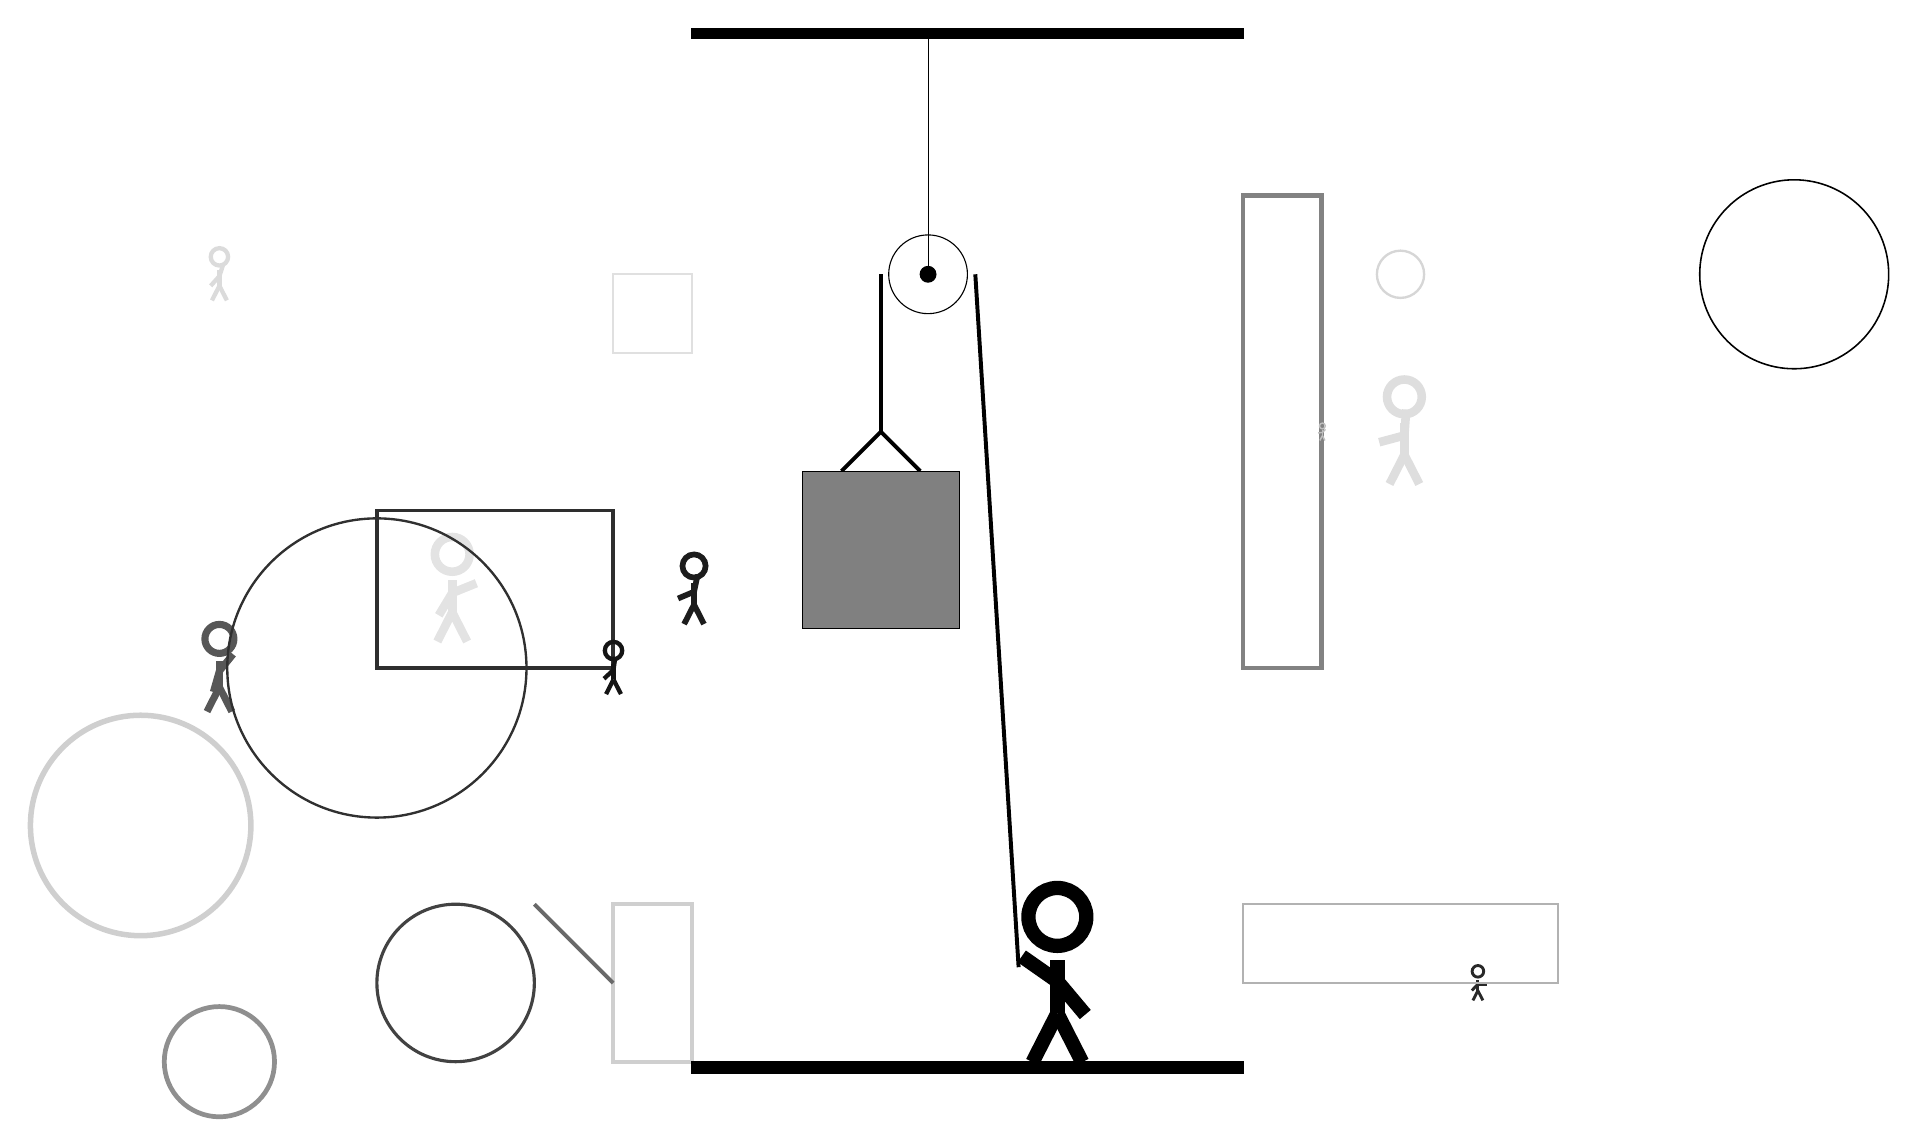
\begin{tikzpicture}
		%%%%% START %%%%%
		
		\draw[fill=black] (-2, 10) rectangle (5, 10.125);
		
		\draw (1, 7) circle (0.5);
		\draw[fill=black] (1, 7) circle (0.1);
		\draw (1, 10) -- (1, 7);
		
		\draw[line width=0.5mm] (-0.1, 4.5) -- (0.4, 5.0) -- (0.9, 4.5);
		\draw[fill=black!50] (-0.6, 4.5) rectangle (1.4, 2.5);
		
		\draw[line width=0.5mm] (0.4, 7) -- (0.4, 5.0);
		\centerarc[line width=0.5mm](1, 7)(0:180:0.6);
		\draw[line width=0.5mm](1.6, 7) -- (2.15, -1.8);
		
		\draw[line width=0.3mm, color=black!12] (-3, 7) rectangle (-2, 6);
		
		\draw [line width=0.7mm, color=black!19](-9, 0) circle (1.4);
		\draw [line width=0.2mm, color=black!100](12, 7) circle (1.2);
		\draw[line width=0.6mm, color=black!49] (6, 8) rectangle (5, 2);
		
		\node[line width=0.2mm, color=black!11] at (-5, 3) {\Strichmaxerl[6][59][22]};
		\draw [line width=0.6mm, color=black!44](-8, -3) circle (0.7);
		\draw[line width=0.5mm, color=black!19] (-3, -1) rectangle (-2, -3);
		
		\node[line width=0.3mm, color=black!25] at (6, 5) {\Strichmaxerl[1][8][45]};
		\draw [line width=0.4mm, color=black!74](-5, -2) circle (1.0);
		
		\node[line width=0.2mm, color=black!84] at (8, -2) {\Strichmaxerl[2][46][0]};
		\node[line width=0.7mm, color=black!66] at (-8, 2) {\Strichmaxerl[5][74][51]};
		\draw[line width=0.5mm, color=black!82] (-3, 2) rectangle (-6, 4);
		\draw[line width=0.3mm, color=black!30] (5, -2) rectangle (9, -1);
		
		\draw[line width=0.5mm, color=black!59](-3, -2) -- (-4, -1);
		\node[line width=0.2mm, color=black!89] at (-2, 3) {\Strichmaxerl[4][23][78]};
		\node[line width=0.4mm, color=black!14] at (-8, 7) {\Strichmaxerl[3][48][72]};
		
		\node[line width=0.7mm, color=black!13] at (7, 5) {\Strichmaxerl[6][15][86]};
		\node[line width=0.2mm, color=black!92] at (-3, 2) {\Strichmaxerl[3][43][82]};
		\draw [line width=0.3mm, color=black!81](-6, 2) circle (1.9);
		\draw [line width=0.3mm, color=black!16](7, 7) circle (0.3);
		
		\node at (2.6, -1.9) {\Strichmaxerl[10][-35][-50]};
		
		\draw[fill=black] (-2, -3) rectangle (5, -3.15);
		
		%%%%% END %%%%%
	\end{tikzpicture}
\end{document}